\documentclass[11pt]{article}
\usepackage[margin=1in]{geometry}
\usepackage{graphicx}
\usepackage{booktabs}
\usepackage{longtable}
\usepackage{array}
\usepackage{float}
\usepackage{hyperref}
\usepackage{tabularx}
\title{Frozen Baseline Review Report}
\author{Round 14 packaging pass}
\date{}
\begin{document}
\maketitle

\section{Executive Summary}
This report freezes the pre-improvement baseline before any future algorithm-strengthening work. The current benchmark inventory contains 11 packaged experiment runs: 2 exact, 4 epsilon-certified, 5 smoke-only, and 0 failed. The validation chain from reference disaster primal through the production Benders engine is already built and individually checked, but the harder exact-mode convergence cases remain non-certified.

\begin{itemize}
\item Exact results currently cover the fixed disaster primal/dual reference chain, the normal-only direct master baselines, and selected tiny or longer-budget exact-mode Benders diagnostics.
\item Epsilon-certified results are bounded certificates relative to their chosen tolerance; they are not exact-zero convergence.
\item Smoke-only runs remain visible and are not promoted into certified evidence.
\item Default \texttt{runtime\_12} remains a local directional benchmark and is not numerically paper-Table-II comparable.
\end{itemize}

\section{Current Frozen Contract}
\begin{itemize}
\item Source-of-truth hierarchy: frozen specs under \texttt{docs/spec/}, validated round reports under \texttt{docs/reports/}, human-facing interpretation packs under \texttt{docs/analysis\_packs/}, and current packaged outputs under \texttt{results/}.
\item Explicit critical-bus freeze for this report: \texttt{[2, 5, 8, 11, 14, 17, 20, 23, 26, 29, 32]}.
\item \texttt{smoke\_only} means a bounded directional run that is not certified evidence.
\item \texttt{epsilon\_certified} means the run stopped with a proved violation upper bound below the configured epsilon, not exact zero.
\item The paper-like family is an approximation layer built from local config overrides, not paper-number reproduction.
\end{itemize}

\section{Validation Chain Summary}
\begin{table}[htbp]
\centering
\footnotesize
\setlength{\tabcolsep}{4pt}
\renewcommand{\arraystretch}{1.12}
\caption{Validation chain summary for the frozen pre-improvement baseline.}
\label{tab:validation-chain-summary}
\begin{tabular}{p{0.8cm} p{3.0cm} p{3.0cm} p{7.0cm}}
\hline
Round & Validated layer & Status & Key result \\
\hline
02 & reference disaster primal & exact toy + runtime fixture & Eq. (26)-(32) fixed-(x,delta,b) primal LP validated \\
03 & canonicalizer + auto dual & exact objective/KKT matching & mechanical canonicalization and auto-dual agree with primal \\
04 & paper dual & exact samplewise decomposition & beta/gamma/phi decomposition matches primal/auto-dual \\
05 & separation oracles & exact tiny validation & outage enumeration, budget support, outer-DRO LP, separation exactness \\
05.5 & separation hardening & coefficient/model-shape validation & runtime bounds and edge-case checks added without changing math \\
06 & first-stage + normal block & toy-case + runtime-smoke validated & Eq. (10)-(25) production blocks built and checked \\
06.5 & unit/interface hardening & analytic Eq. (24) guard & voltage-drop scaling and first-stage API protected by tests \\
07 & fixed-cut master & toy-case + runtime-smoke validated & restricted master for Eq. (33), (37)-(39) built \\
07.5 & master/cut interface & real-cut interface hardened & paper-dual decomposition enters master without flattening \\
08 & single generated cut step & one-step efficacy validated & master -> separation -> cut -> master path built \\
09 & full Benders engine & tiny exact + runtime smoke & iterative Benders loop validated against brute force on tiny case \\
10 & independent disaster exact oracle & tiny cross-check + readiness & primal-exact disaster oracle agrees with production tiny path \\
11 & experiment interpretation pack & packaging only & benchmark packaging and explicit validation labels introduced \\
12 & paper-style experiment pack & packaging only & paper-like and runtime-directional families packaged with failures visible \\
12.5 & convergence diagnostics & diagnostic only & exact\_zero / epsilon\_stop / max\_iter\_noncert separated \\
13 & cut-process diagnostics & diagnostic only & repeated outages observed; exact duplicate structured cuts not observed \\
\hline
\end{tabular}
\end{table}


\section{Benchmark Experiment Summary}
Certified-small family (regenerated in this round because the Round 12 packaged outputs no longer carried those rows separately):
\begin{itemize}
\item none
\end{itemize}

Paper-like family:
\begin{itemize}
\item integrated\_mainline\_paper\_like: validation=epsilon\_certified, stop=certified\_epsilon, construction=171,730.136, weighted normal=13,035,357.592, disaster master=0.000000
\item normal\_only\_paper\_like: validation=exact, stop=direct\_optimal, construction=171,760.064, weighted normal=18,622,035.264, disaster master=0.000000
\item disaster\_only\_paper\_like: validation=smoke\_only, stop=max\_iterations, construction=23,113.825, weighted normal=0.000000, disaster master=3,709.868
\item deterministic\_mean\_value\_paper\_like: validation=epsilon\_certified, stop=certified\_epsilon, construction=171,730.136, weighted normal=13,035,357.592, disaster master=0.000000
\item ev\_penetration\_1\_5x\_paper\_like: validation=epsilon\_certified, stop=certified\_epsilon, construction=262,853.694, weighted normal=17,010,934.514, disaster master=0.000000
\item ev\_penetration\_2\_0x\_paper\_like: validation=epsilon\_certified, stop=certified\_epsilon, construction=305,364.115, weighted normal=25,867,747.207, disaster master=0.000000
\end{itemize}

Runtime12 directional family:
\begin{itemize}
\item integrated\_mainline\_runtime12: validation=smoke\_only, stop=max\_iterations, construction=4,410,273.924, weighted normal=20,506,437.556, disaster master=87.352783
\item normal\_only\_runtime12: validation=exact, stop=direct\_optimal, construction=4,410,273.924, weighted normal=22,784,930.618, disaster master=0.000000
\item deterministic\_mean\_value\_runtime12: validation=smoke\_only, stop=max\_iterations, construction=4,183,374.434, weighted normal=20,674,646.361, disaster master=103.570653
\item ev\_penetration\_1\_5x\_runtime12: validation=smoke\_only, stop=max\_iterations, construction=6,172,481.342, weighted normal=30,577,949.733, disaster master=122.108885
\item ev\_penetration\_2\_0x\_runtime12: validation=smoke\_only, stop=max\_iterations, construction=6,470,032.170, weighted normal=46,930,921.151, disaster master=122.108885
\end{itemize}

Validation labels by packaged experiment run:
\begin{itemize}
\item - `exact`: `normal\_only\_paper\_like`, `normal\_only\_runtime12`
\item - `epsilon\_certified`: `integrated\_mainline\_paper\_like`, `deterministic\_mean\_value\_paper\_like`, `ev\_penetration\_1\_5x\_paper\_like`, `ev\_penetration\_2\_0x\_paper\_like`
\item - `smoke\_only`: `disaster\_only\_paper\_like`, `integrated\_mainline\_runtime12`, `deterministic\_mean\_value\_runtime12`, `ev\_penetration\_1\_5x\_runtime12`, `ev\_penetration\_2\_0x\_runtime12`
\item - `failed`: none
\end{itemize}

\section{IEEE 33-Bus Station Topology Interpretation}
Figures~\ref{fig:runtime12-maps-a} and \ref{fig:runtime12-maps-b} show the runtime12 directional maps in two larger panels, while Figures~\ref{fig:paper123} and \ref{fig:paper456} show the paper-like maps. Critical buses are highlighted explicitly in red. The current baseline supports a careful topological interpretation: integrated and normal-only plans often place direct capacity at or near critical buses, fast-charger hubs concentrate on a smaller subset of opened buses, and EV-penetration expansion is monotone in buildout. None of these plots should be read as paper-number reproduction.

\begin{figure}[H]
\centering
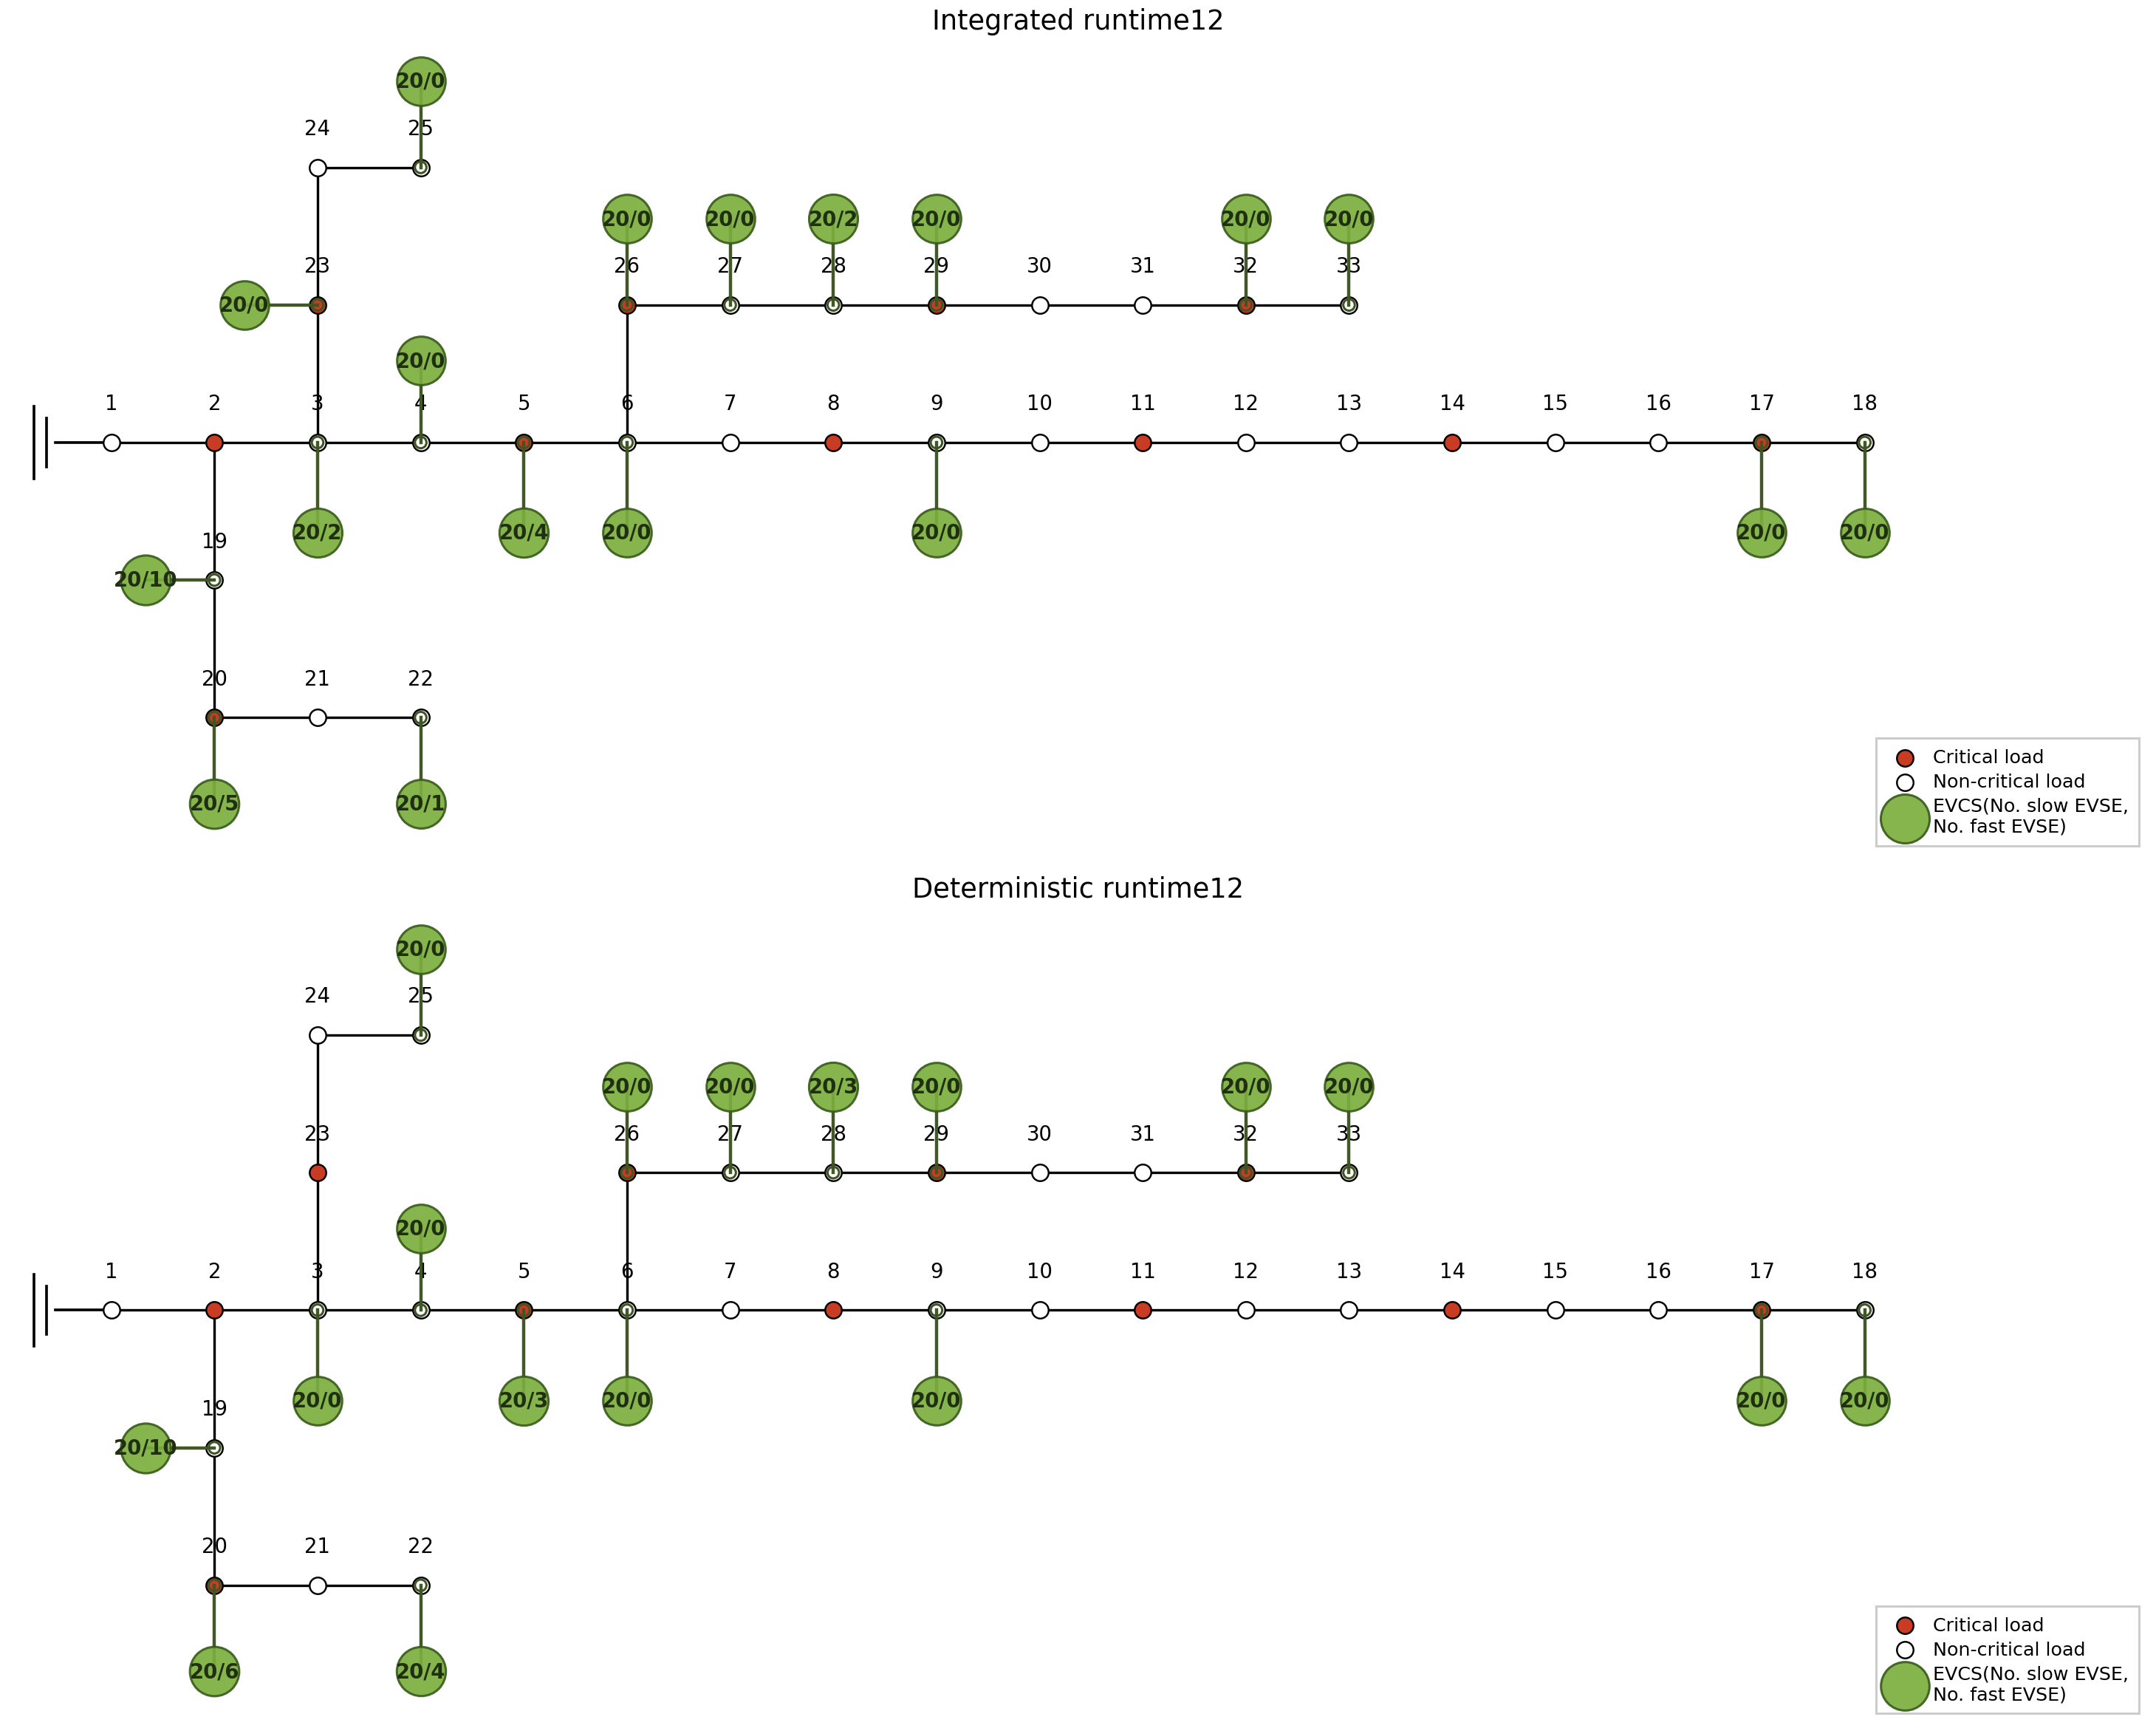
\includegraphics[width=0.82\textwidth,height=0.82\textheight,keepaspectratio]{figures/baseline/ieee33_runtime12_directional_maps_a.png}
\caption{Runtime12 directional topology maps, part 1: integrated and deterministic runs.}
\label{fig:runtime12-maps-a}
\end{figure}

\begin{figure}[H]
\centering
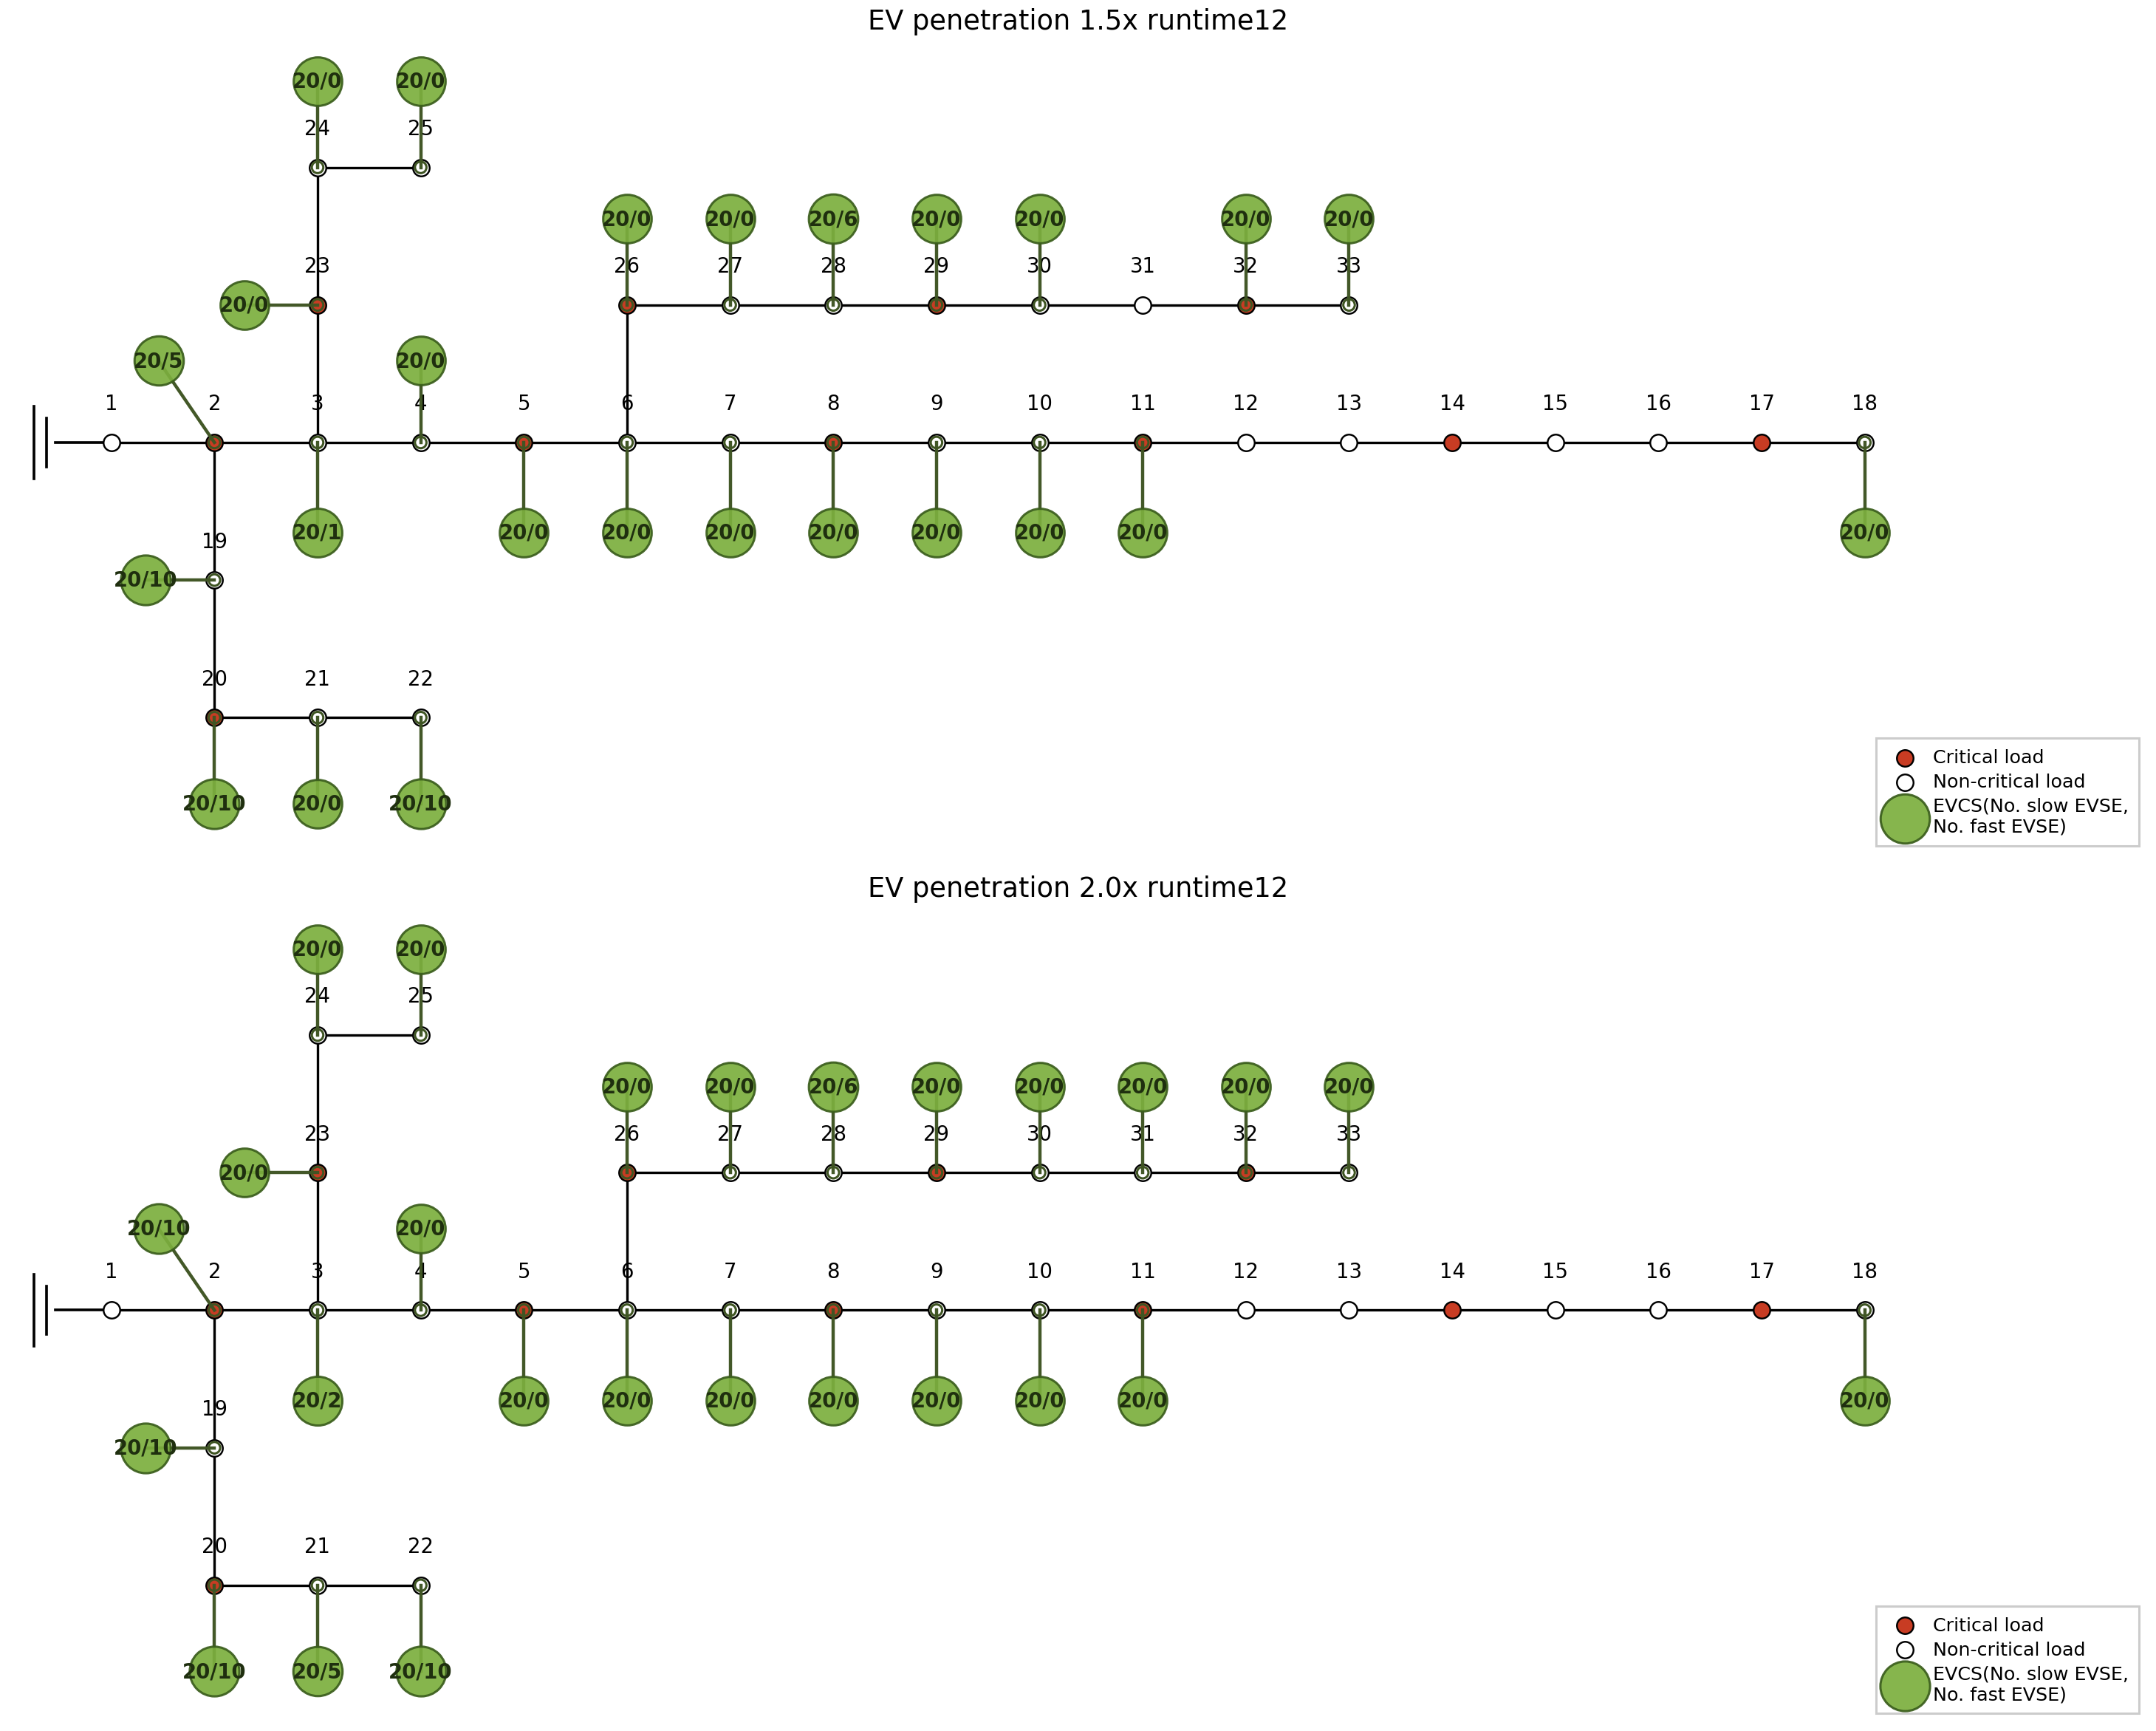
\includegraphics[width=0.82\textwidth,height=0.82\textheight,keepaspectratio]{figures/baseline/ieee33_runtime12_directional_maps_b.png}
\caption{Runtime12 directional topology maps, part 2: EV-penetration runs.}
\label{fig:runtime12-maps-b}
\end{figure}

\begin{figure}[H]
\centering
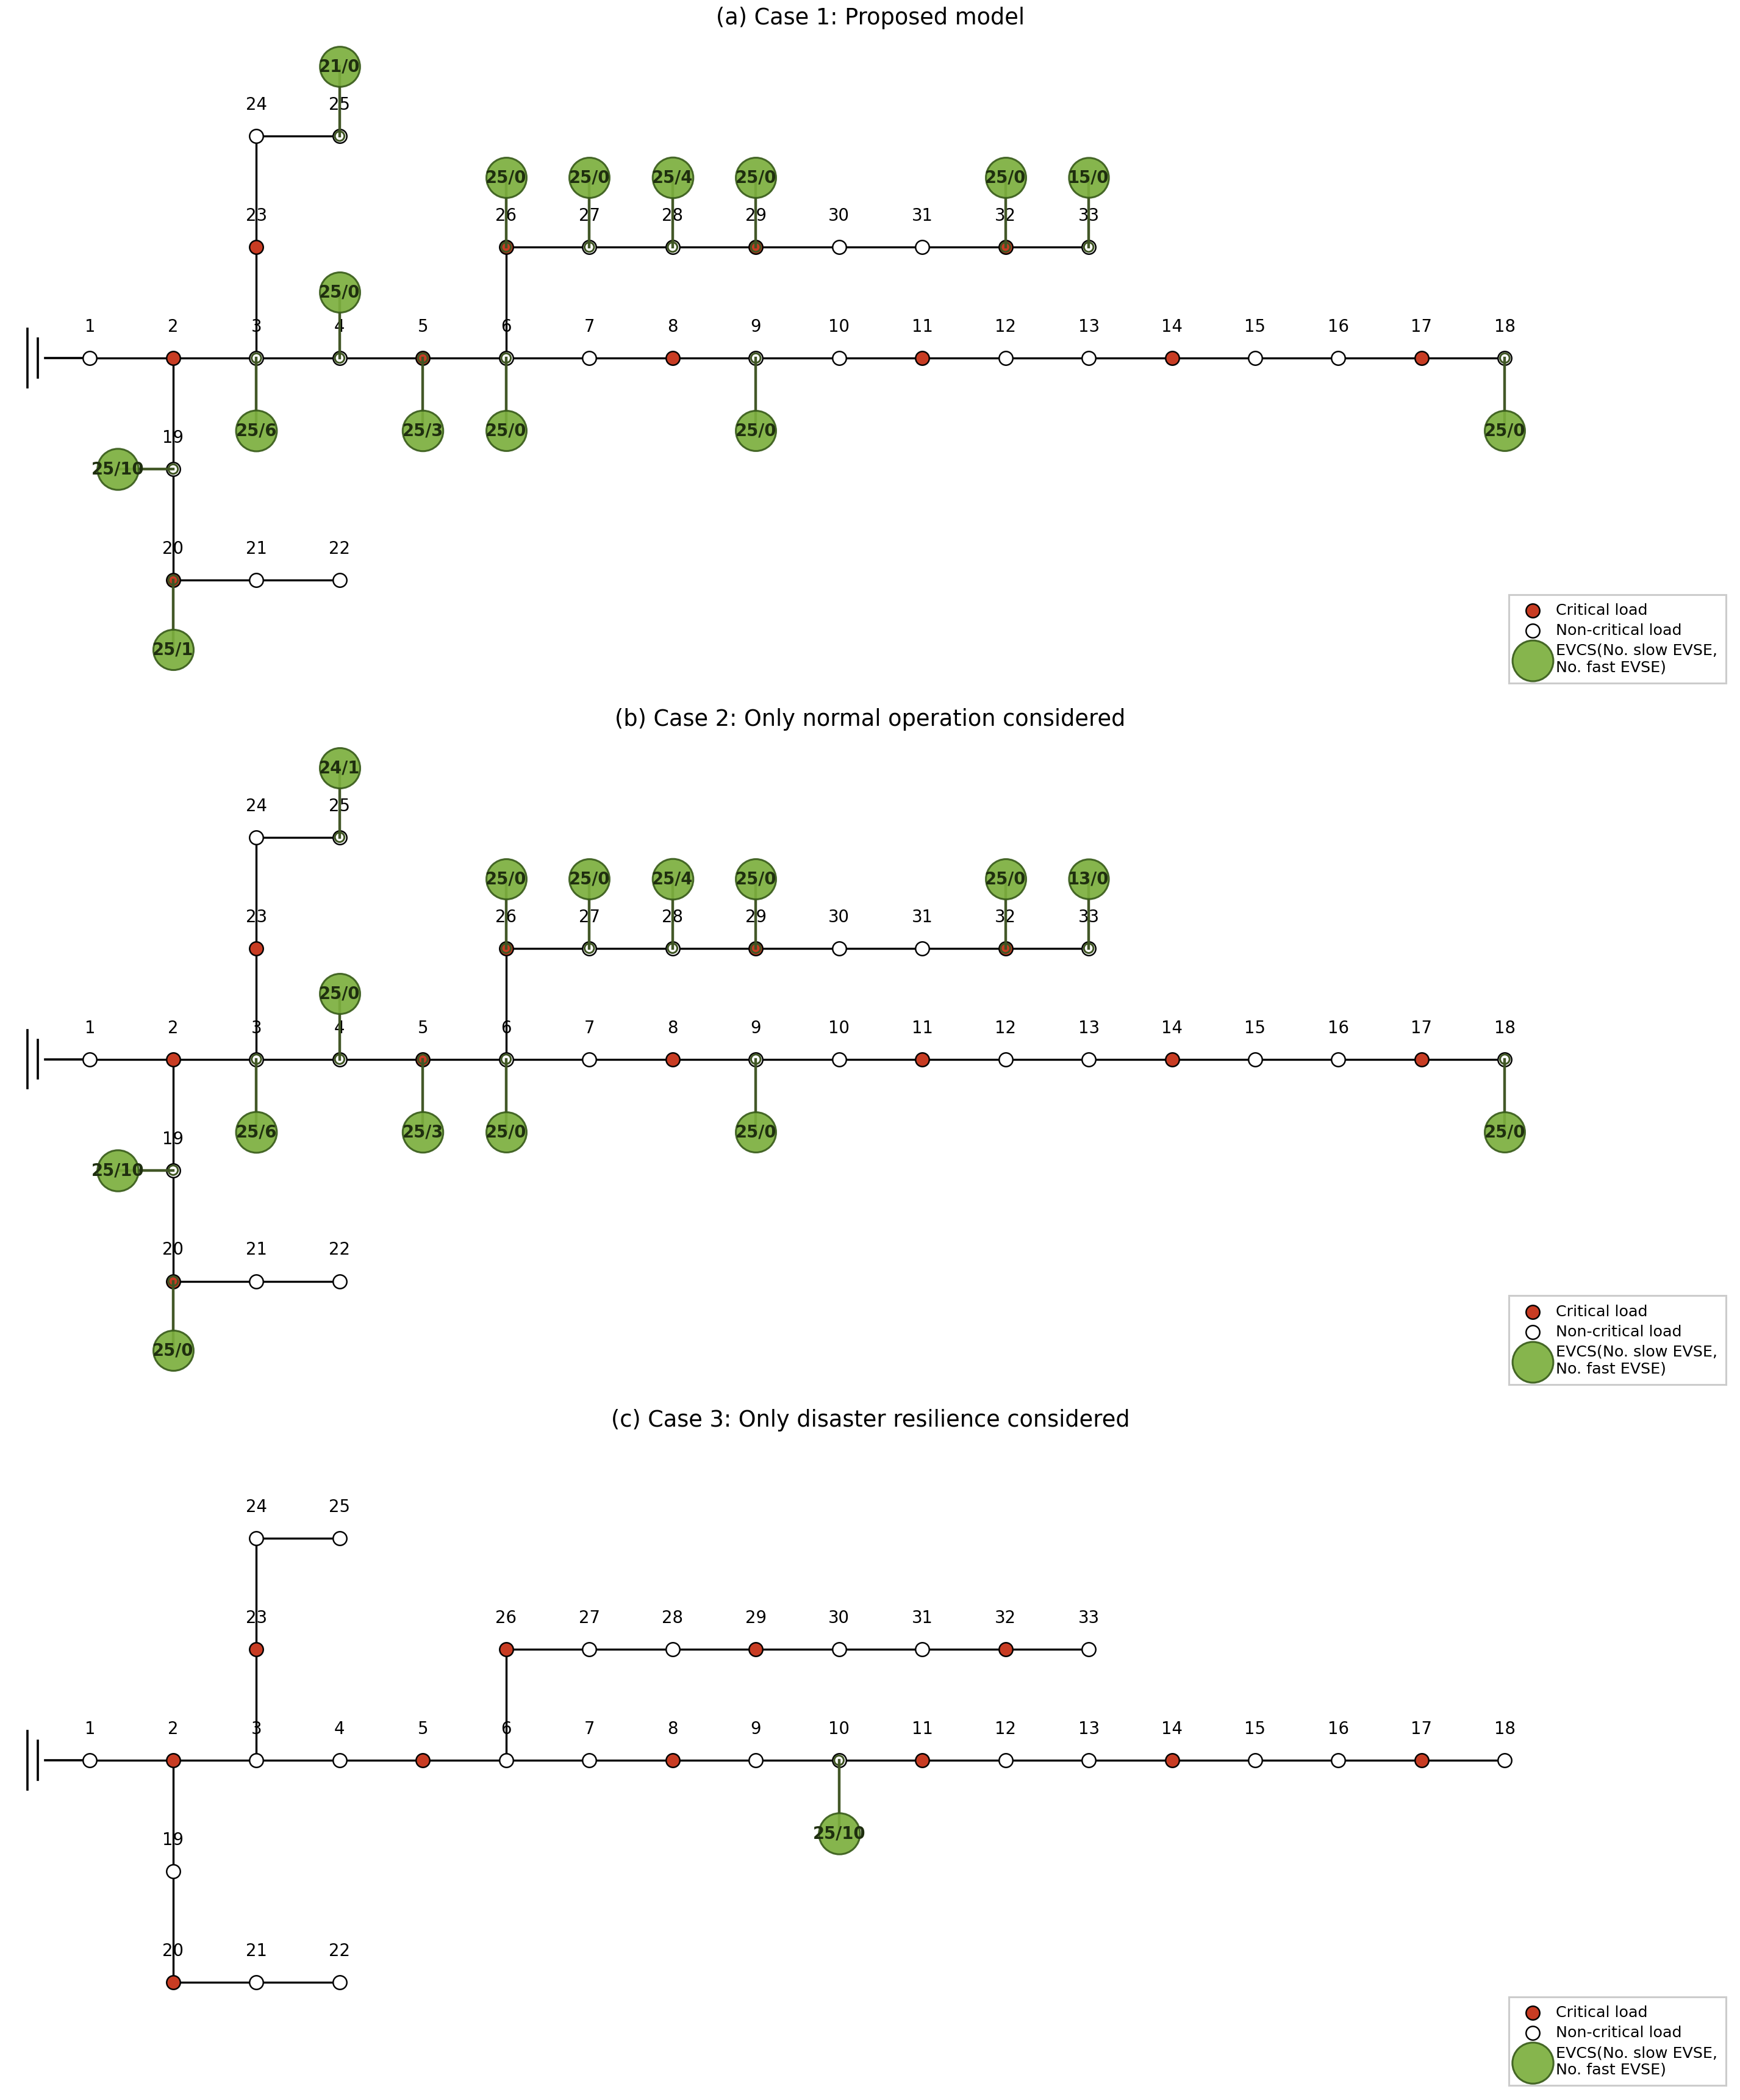
\includegraphics[width=0.88\textwidth,height=0.88\textheight,keepaspectratio]{figures/baseline/ieee33_paper_like_maps_case123.png}
\caption{Paper-like case 1/2/3 topology maps: integrated, normal-only, disaster-only.}
\label{fig:paper123}
\end{figure}

\begin{figure}[H]
\centering
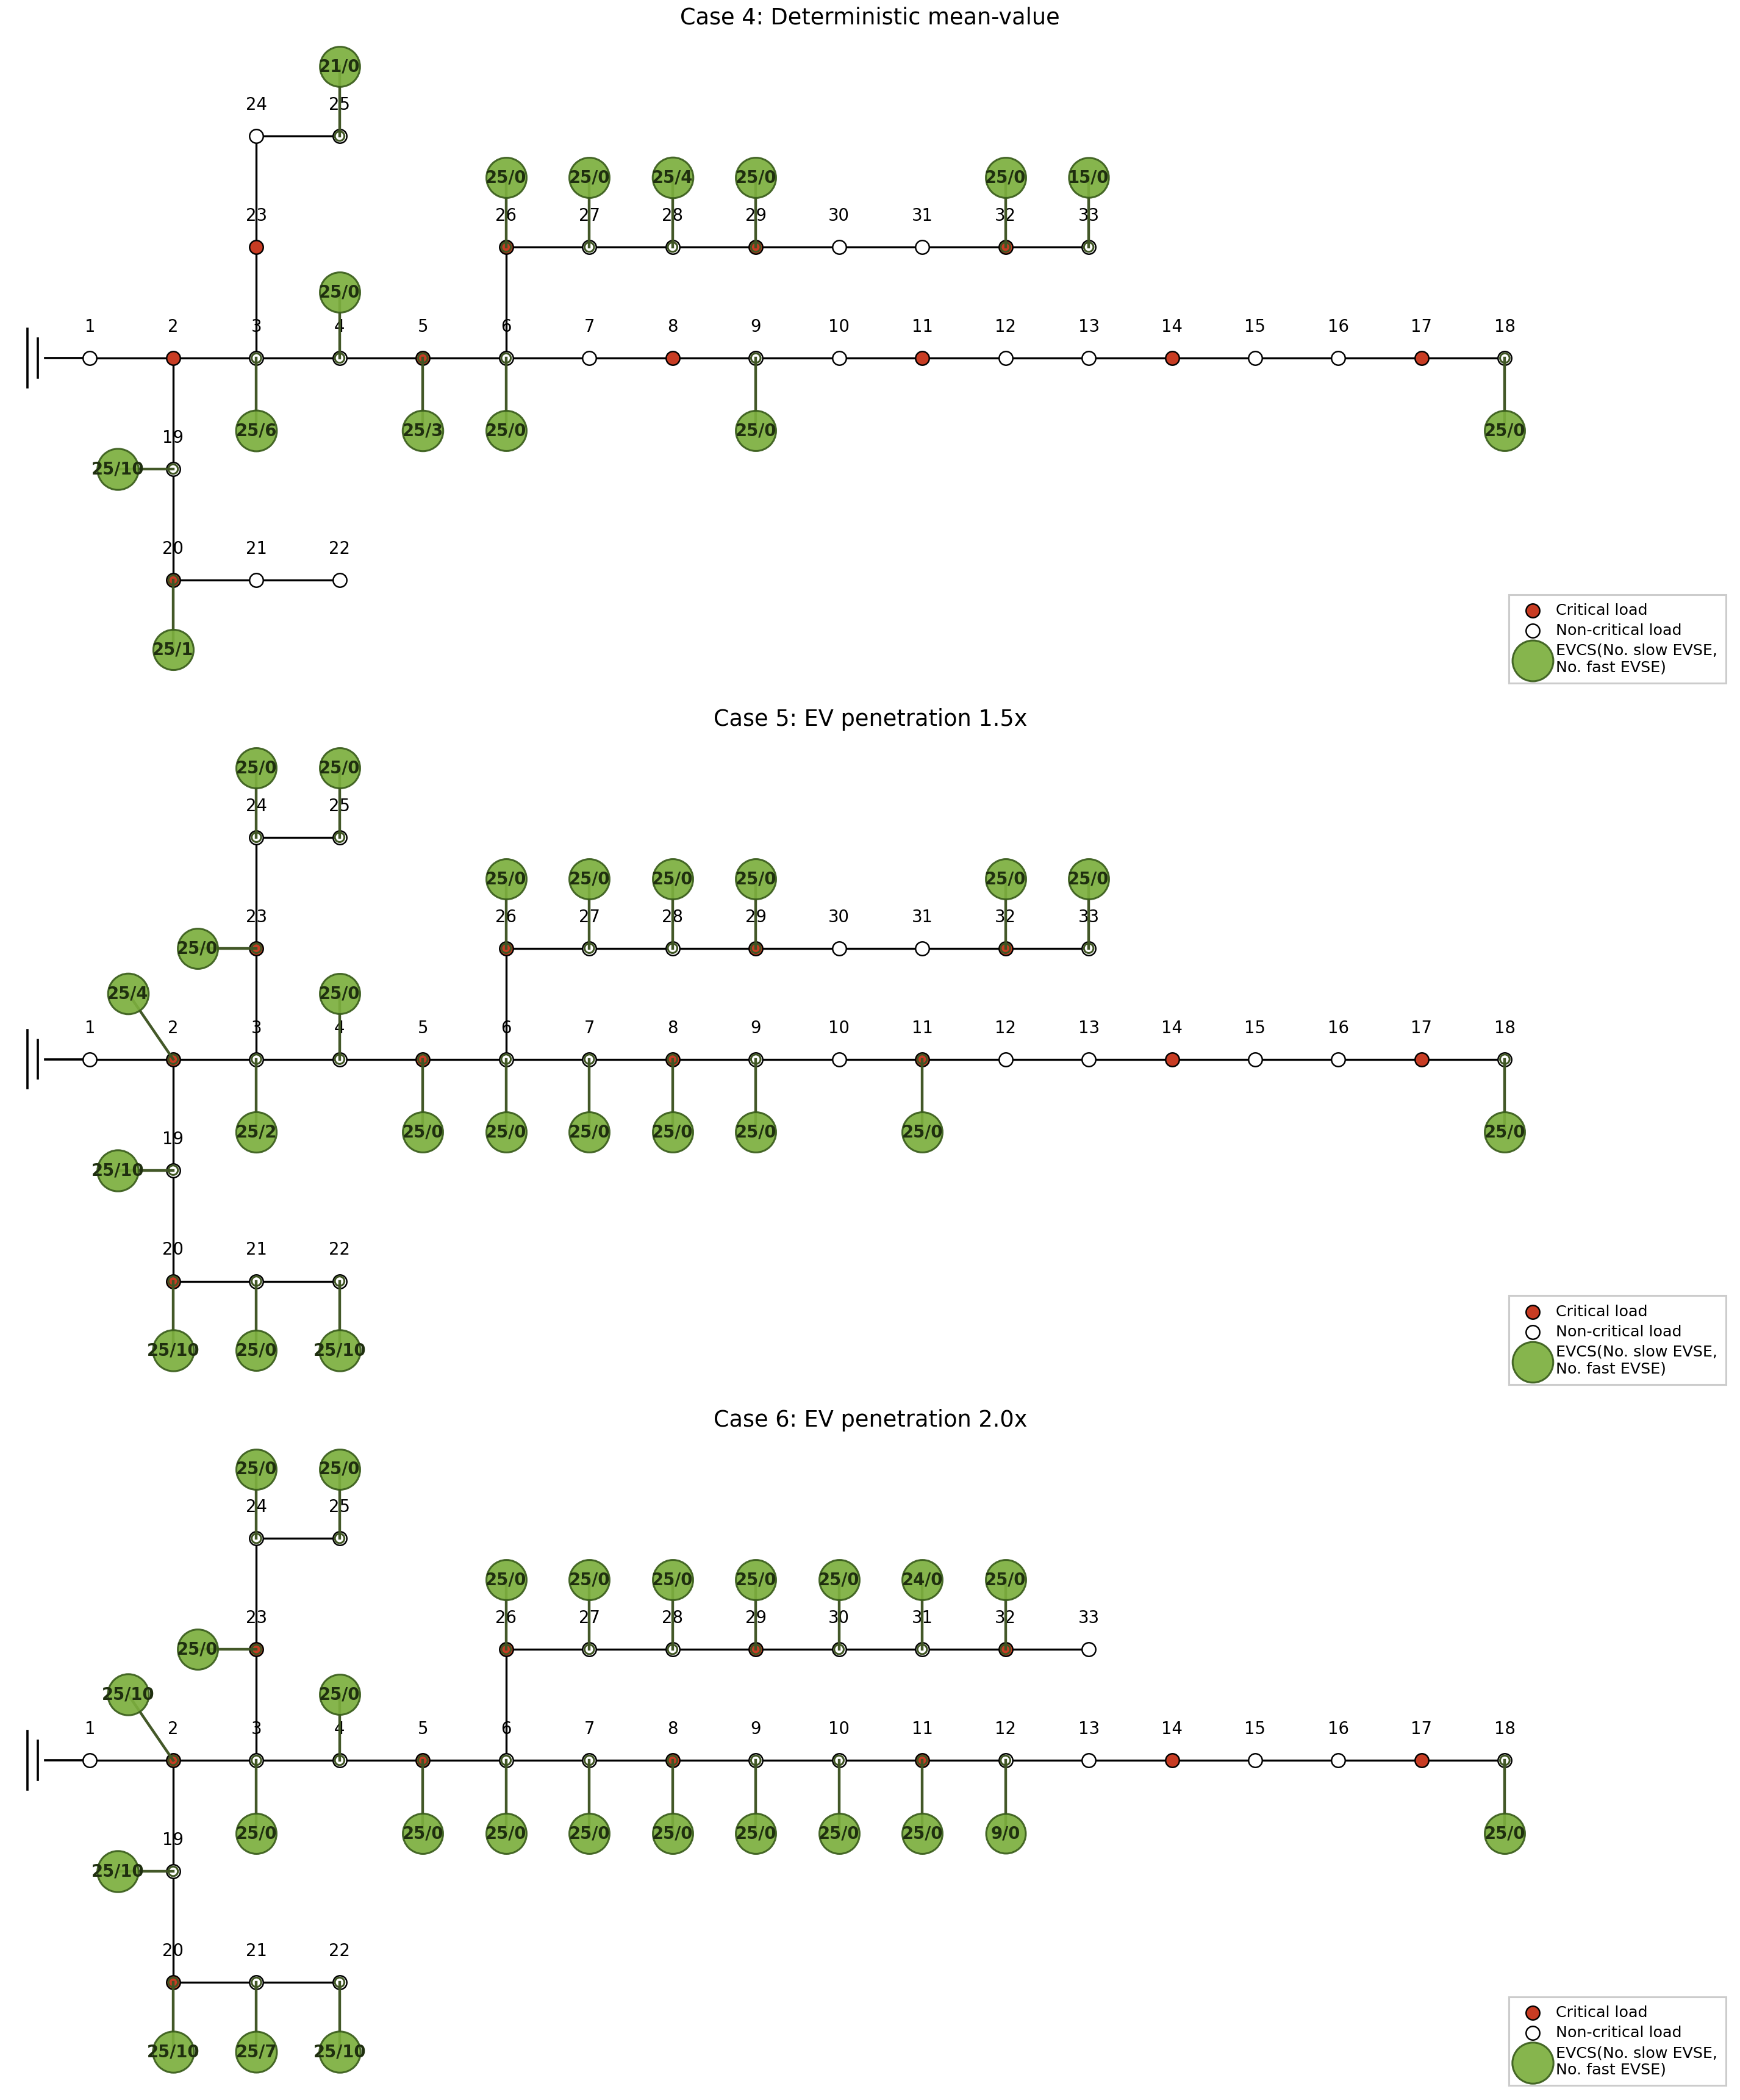
\includegraphics[width=0.88\textwidth,height=0.88\textheight,keepaspectratio]{figures/baseline/ieee33_paper_like_maps_case4_56.png}
\caption{Paper-like case 4/5/6 topology maps: deterministic mean-value and EV-penetration cases.}
\label{fig:paper456}
\end{figure}

\section{Objective Decomposition}
Figure~\ref{fig:obj-components} uses the weighted normal term consistently and keeps the unweighted normal term out of the main stacked chart. Cross-family ranking by raw total objective is intentionally avoided in the safer benchmark comparison view of Figure~\ref{fig:safe-benchmark}.

\begin{figure}[H]
\centering
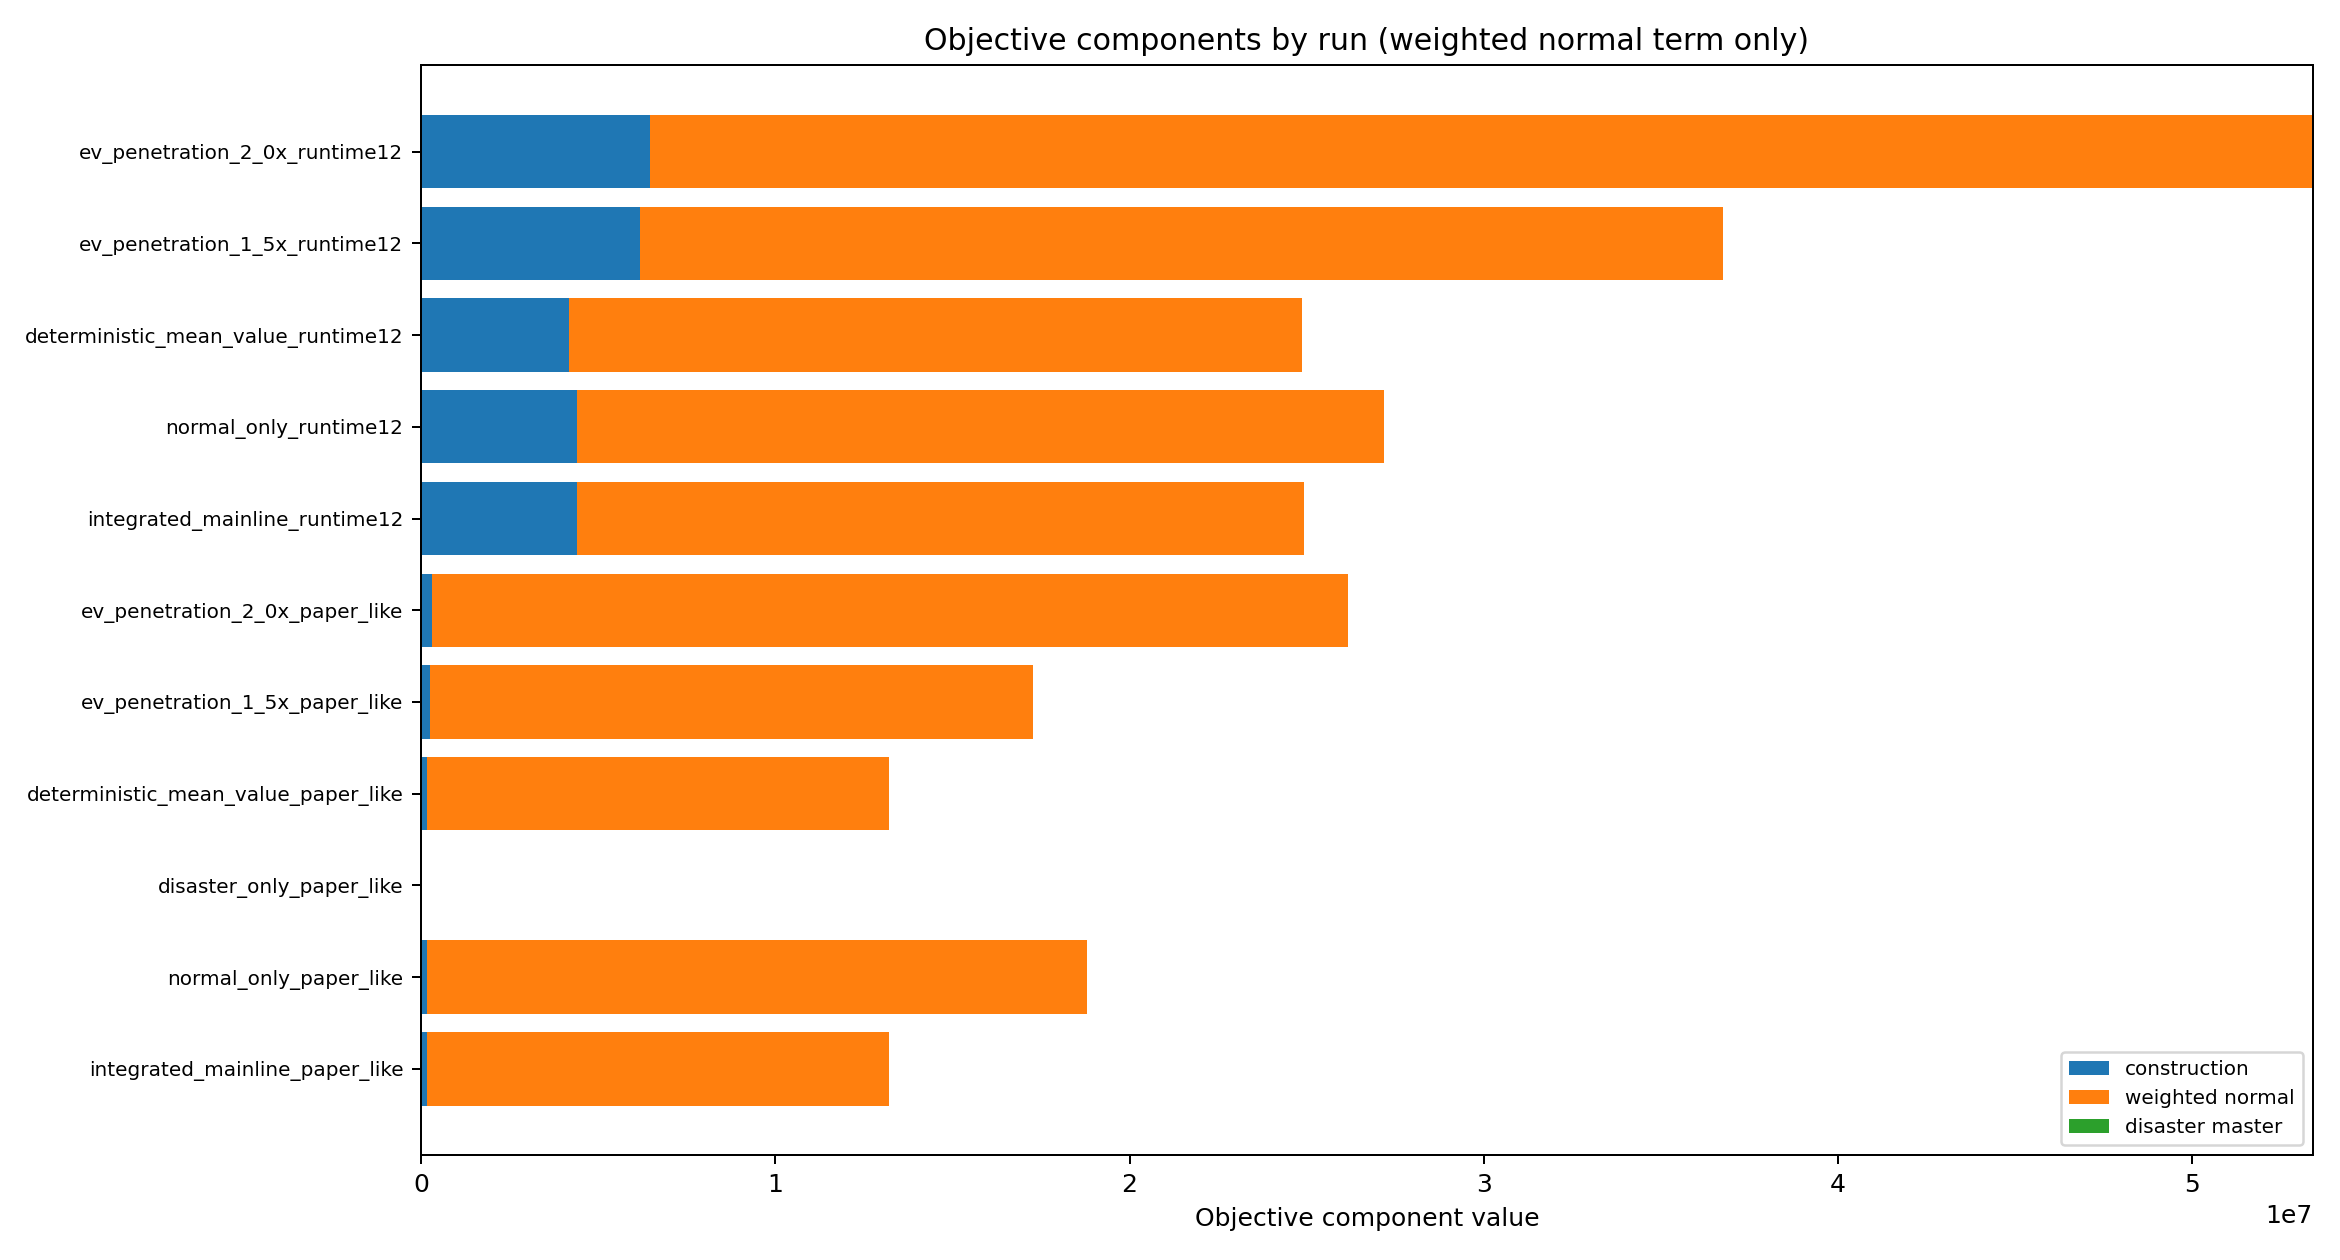
\includegraphics[width=\textwidth]{figures/baseline/objective_components_by_run.png}
\caption{Construction, weighted normal term, and disaster master term by run.}
\label{fig:obj-components}
\end{figure}

\begin{figure}[H]
\centering
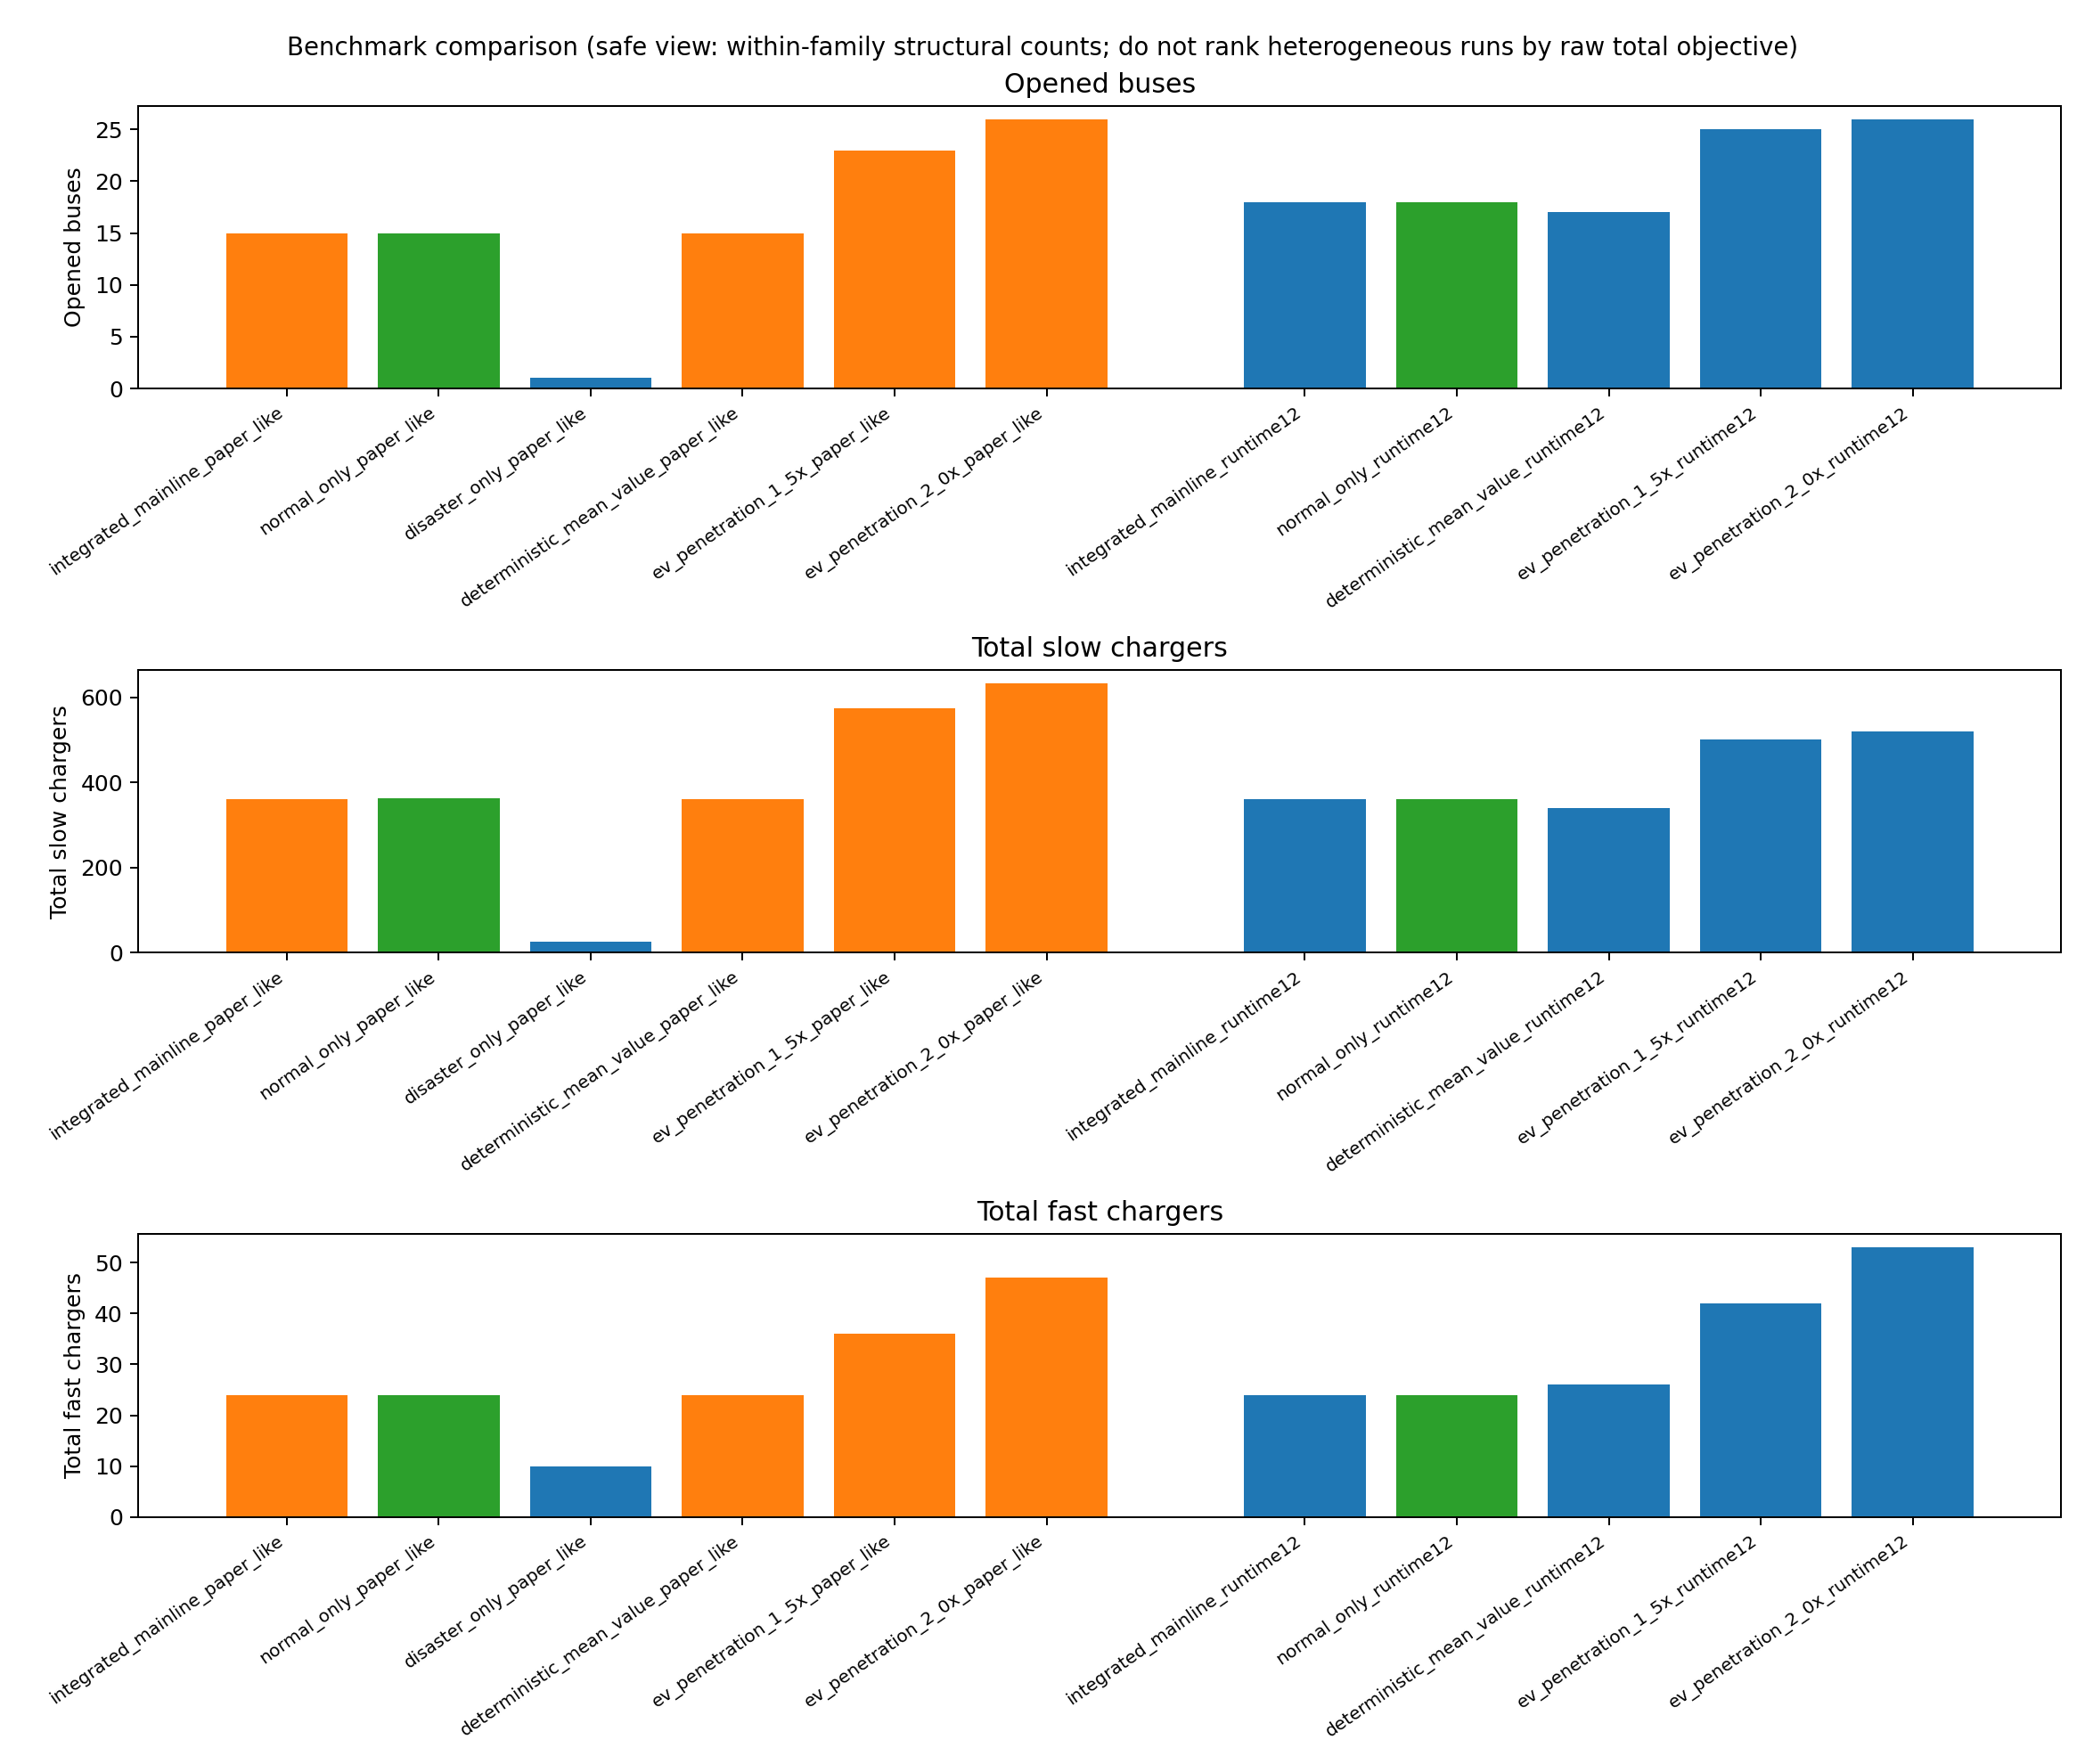
\includegraphics[width=\textwidth]{figures/baseline/benchmark_comparison_safe.png}
\caption{Safer benchmark comparison based on structural counts within each family.}
\label{fig:safe-benchmark}
\end{figure}

\section{Convergence / Non-Certification Diagnostics}
The convergence and cut-process diagnostics keep non-certified runs visible. Round 12.5 showed that exact-zero, epsilon-stop, and max-iteration non-certification need to be separated explicitly. Round 13 showed repeated outages in several hard cases, while exact duplicate structured cut signatures were not observed.

\begin{itemize}
\item Repeated-outage cases from Round 12.5: integrated\_paper\_like\_exact\_i20\_k2\_a1b1, disaster\_only\_paper\_like\_exact\_i20\_k2\_a1b1.
\item Repeated structured-cut signature cases from Round 12.5: none observed.
\item Hard exact-mode or strengthened diagnostic cases still non-certified: integrated\_paper\_like\_exact\_i10\_k2\_a1b1\_\_baseline, integrated\_paper\_like\_exact\_i20\_k2\_a1b1\_\_baseline, disaster\_only\_paper\_like\_exact\_i5\_k1\_a1b1\_\_baseline, disaster\_only\_paper\_like\_exact\_i20\_k1\_a1b1\_\_baseline, disaster\_only\_paper\_like\_exact\_i5\_k2\_a1b1\_\_baseline, disaster\_only\_paper\_like\_exact\_i20\_k2\_a1b1\_\_baseline, disaster\_only\_paper\_like\_exact\_i40\_k2\_a1b1\_\_baseline, integrated\_runtime12\_exact\_i3\_k3\_a1234b1234\_\_baseline.
\end{itemize}

\begin{figure}[H]
\centering
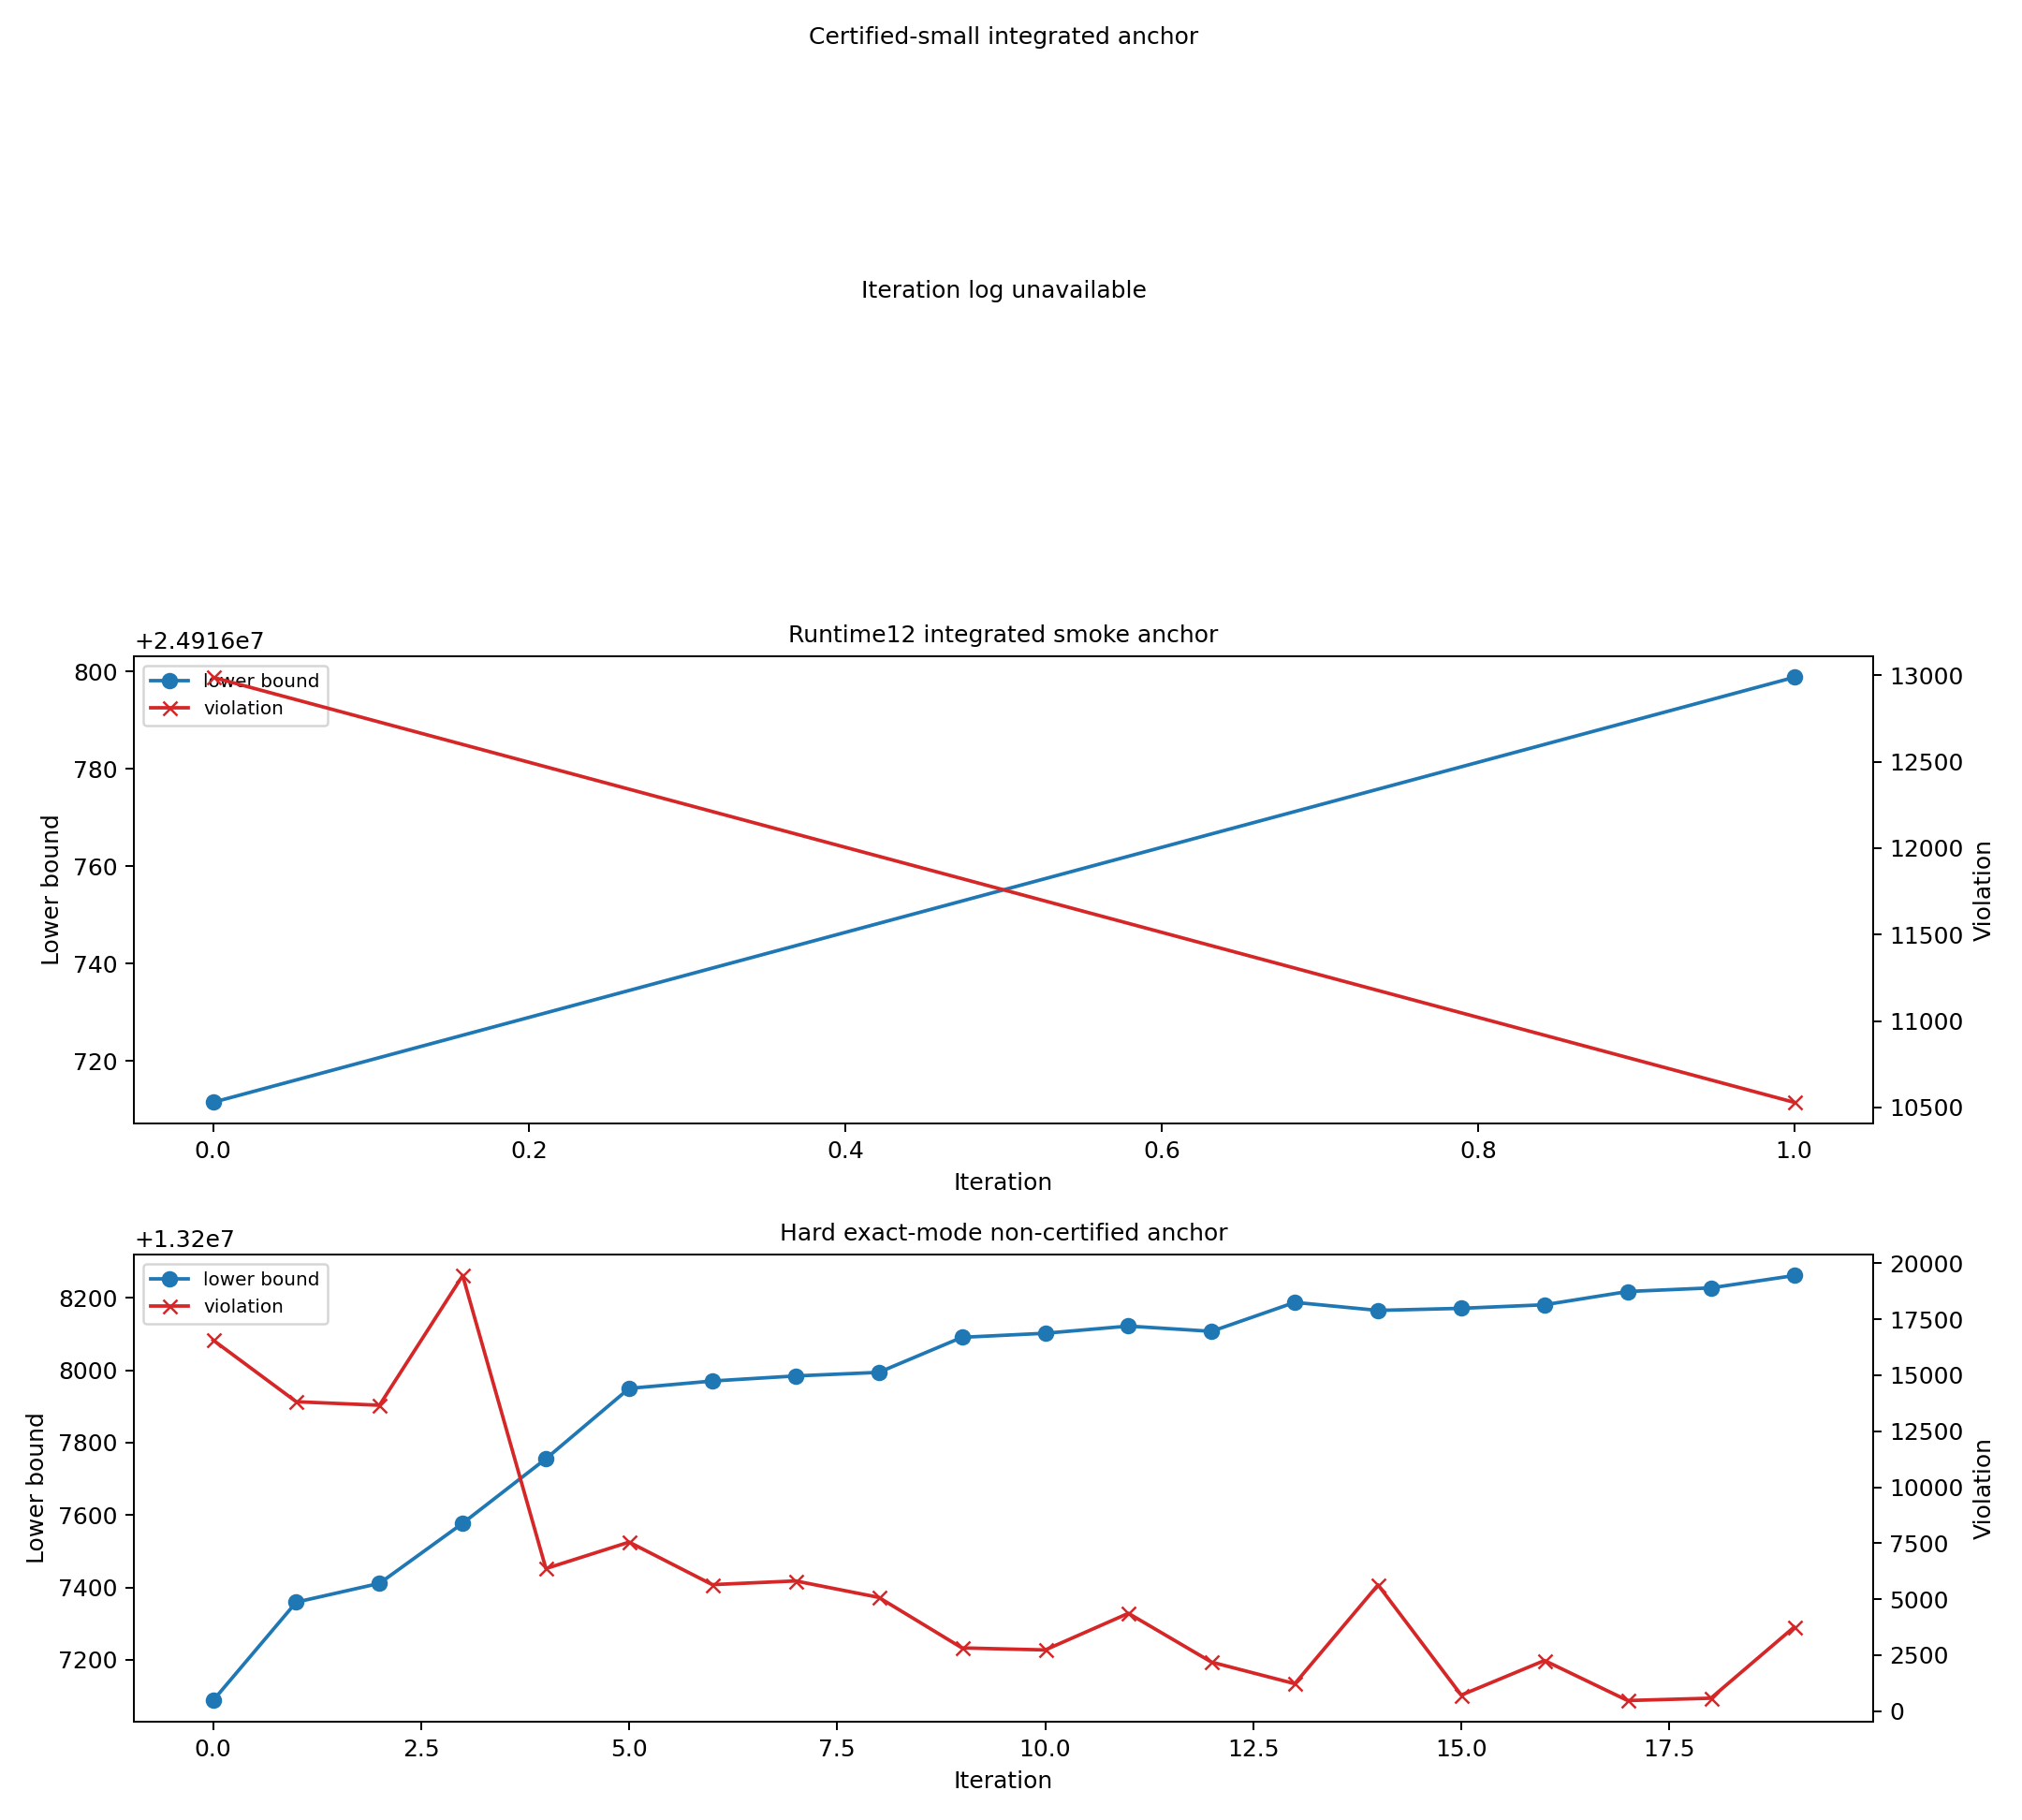
\includegraphics[width=\textwidth]{figures/baseline/iteration_trace_selected.png}
\caption{Selected iteration traces: certified-small anchor, runtime smoke anchor, and hard exact-mode non-certified anchor.}
\end{figure}

\begin{figure}[H]
\centering
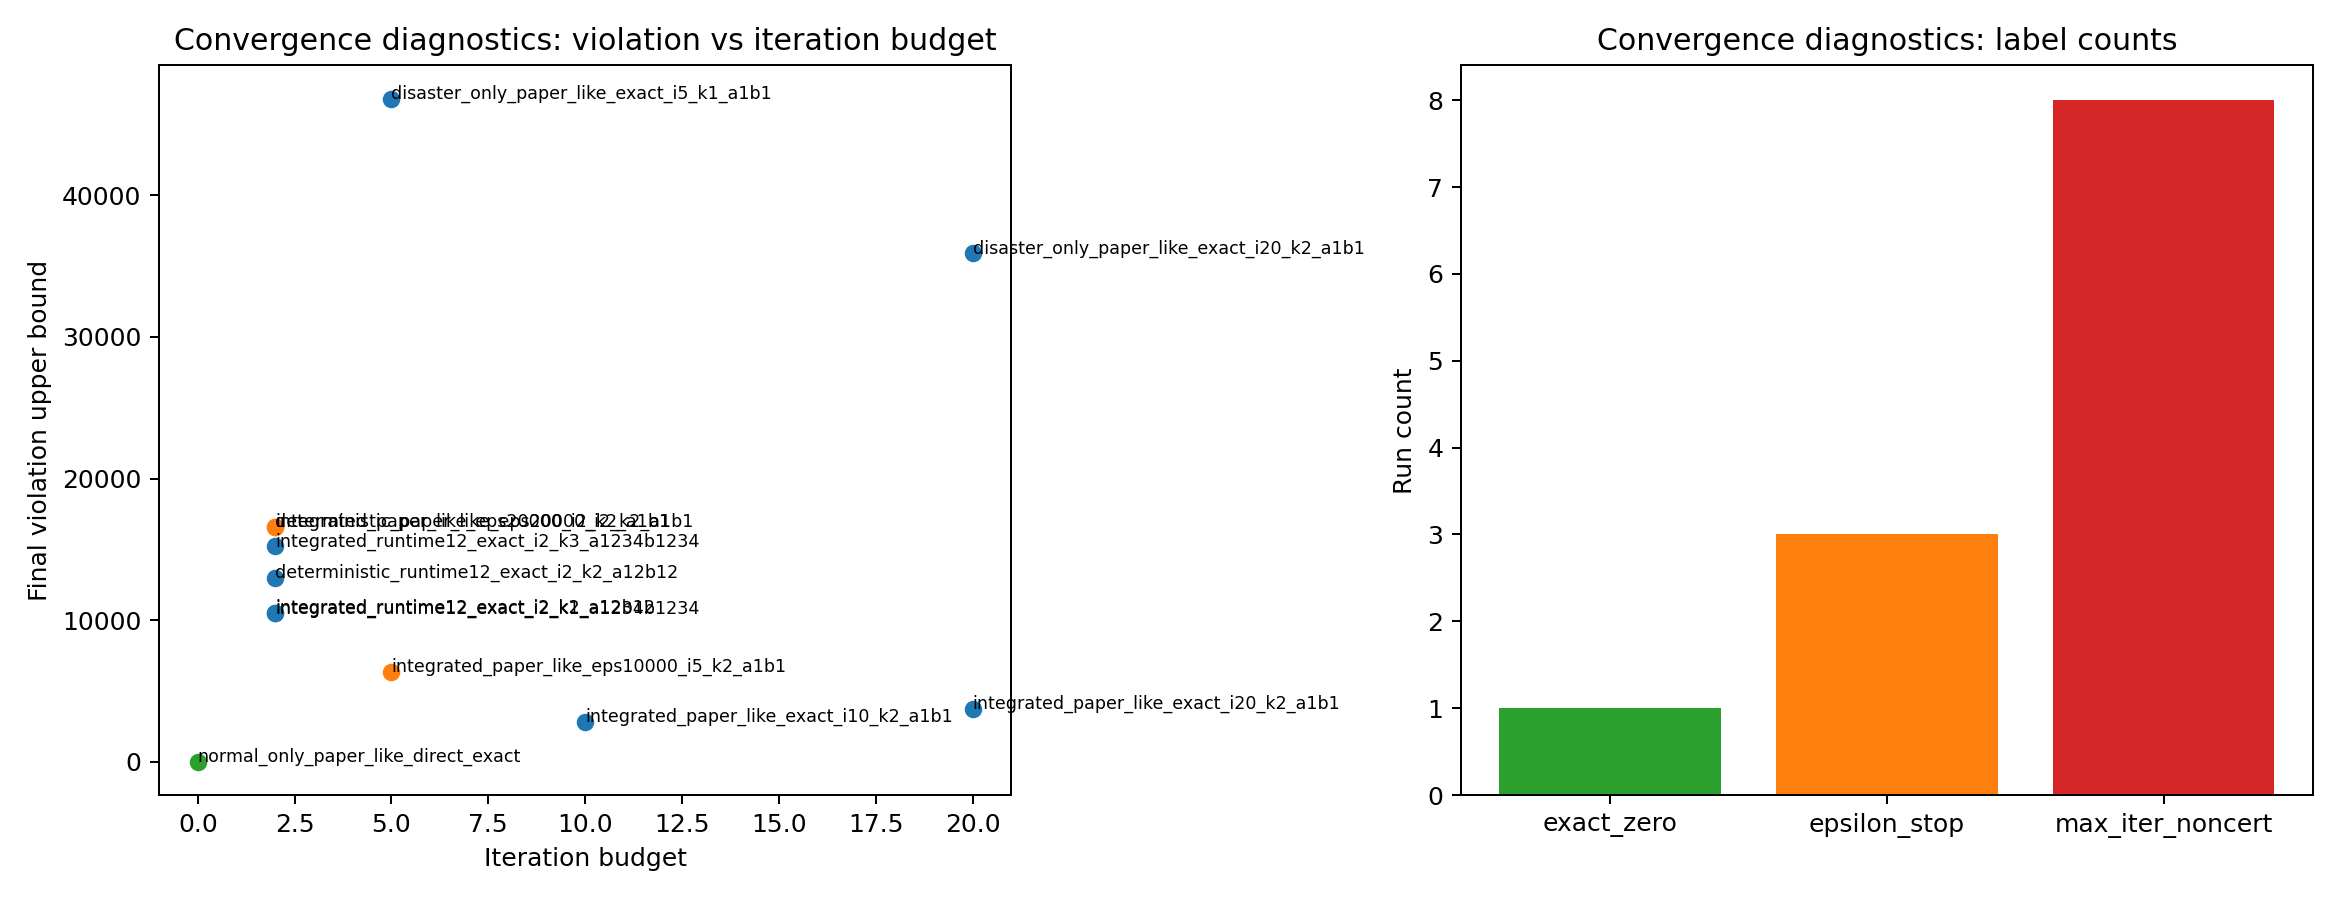
\includegraphics[width=\textwidth]{figures/baseline/convergence_diagnostics_overview.png}
\caption{Round 12.5 convergence-diagnostic overview.}
\end{figure}

\begin{figure}[H]
\centering
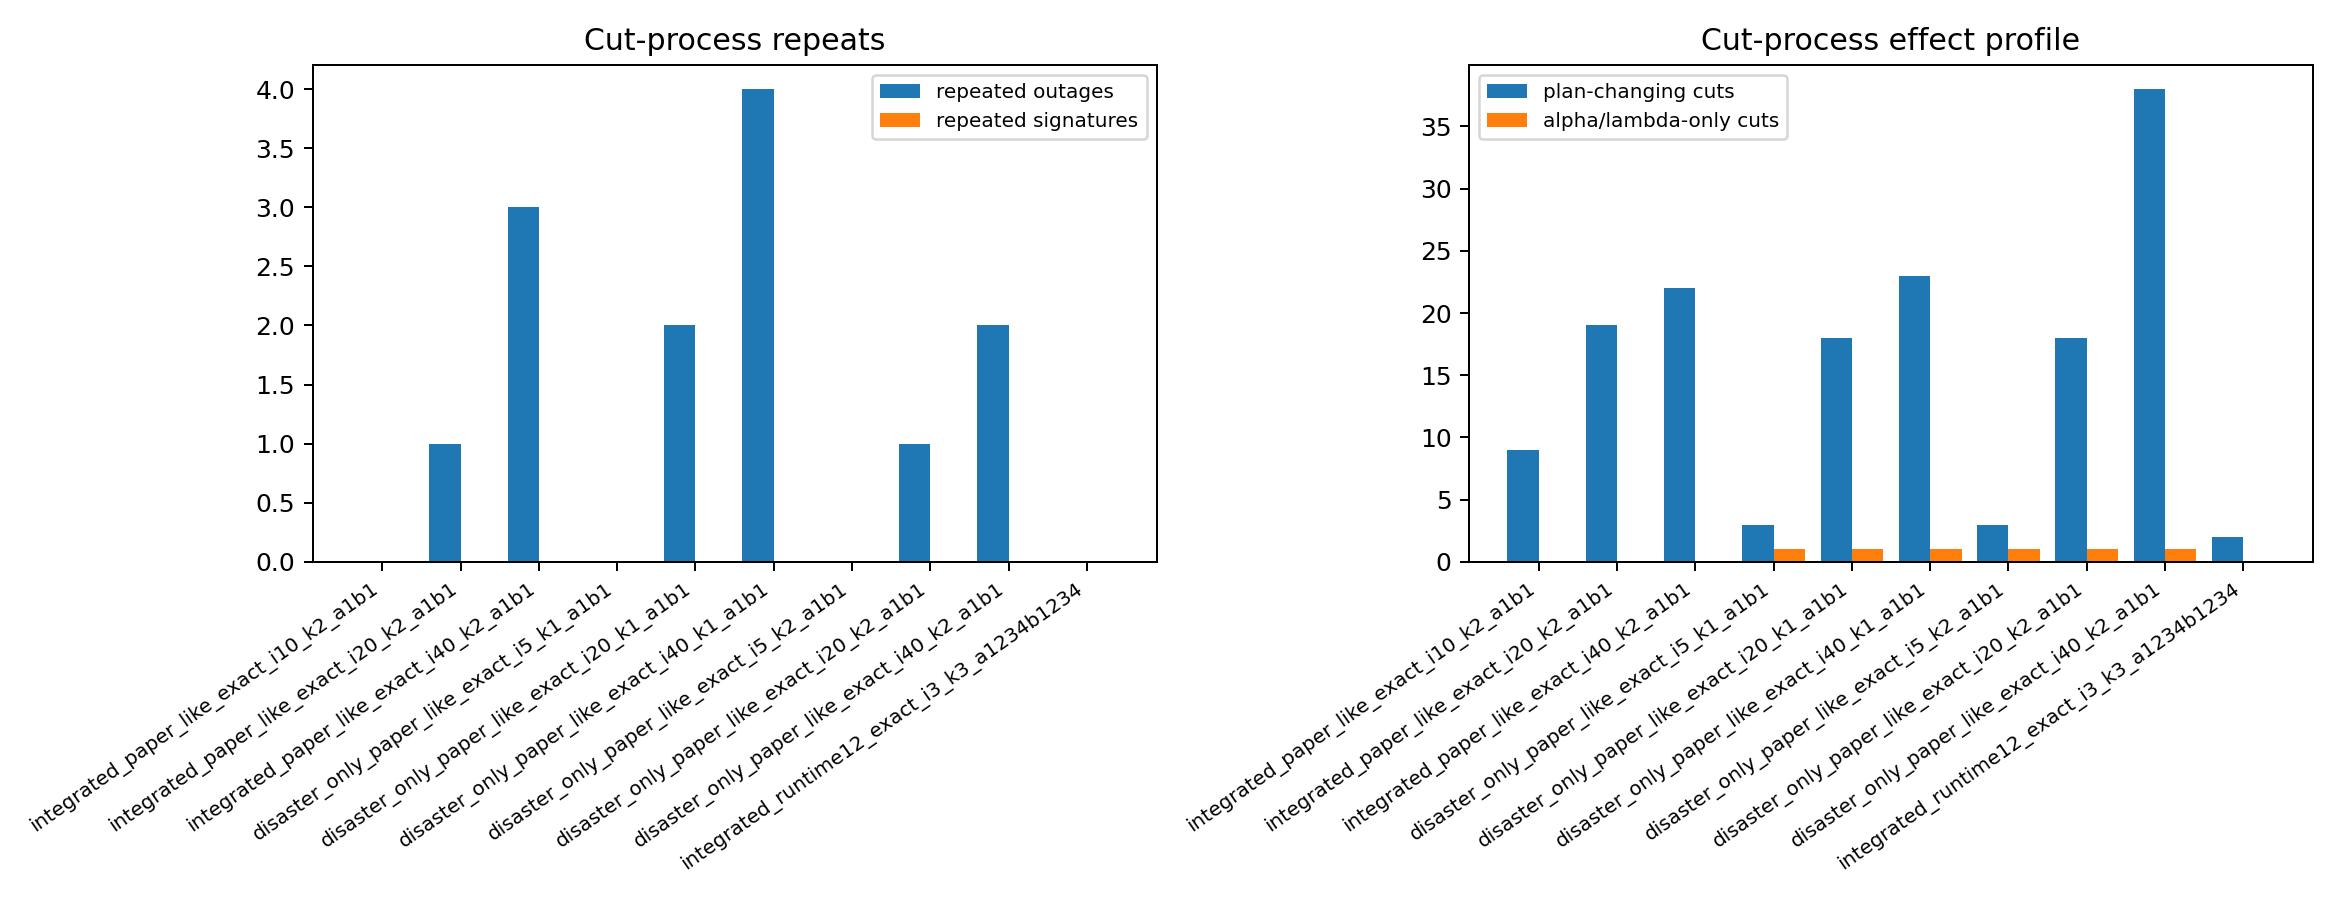
\includegraphics[width=\textwidth]{figures/baseline/cut_process_diagnostics_overview.png}
\caption{Round 13 cut-process overview.}
\end{figure}

\section{Safe Claims vs Unsafe Claims}
\textbf{Safe now.}
\begin{itemize}
\item The reference-to-production validation chain has been individually exercised from the disaster primal through the fixed-cut master and iterative Benders engine.
\item Exact, epsilon-certified, smoke-only, and failed labels are preserved explicitly in the frozen baseline.
\item The current diagnosis points at cut-process effectiveness as the main remaining difficulty in the harder exact-mode runs, not at raw-data loading or a known core-math break.
\end{itemize}

\textbf{Not safe yet.}
\begin{itemize}
\item Default \texttt{runtime\_12} is not paper-Table-II comparable.
\item The paper-like family is not a paper-number reproduction.
\item Heterogeneous benchmark runs should not be ranked by raw total objective without caveats.
\item Hard non-certified exact-mode runs should not be described as converged.
\end{itemize}

\section{Next Improvement Priorities}
\begin{enumerate}
\item Strengthen cut-process effectiveness rather than relabeling smoke-only outcomes.
\item Revisit multi-cut or stabilization ideas only after preserving the current exact/epsilon/smoke discipline.
\item Keep baseline archive, anchor reruns, and honest non-certification visibility intact during future improvement rounds.
\end{enumerate}

\section*{Anchor Consistency Checks}
The round reran three anchors against archived/current baselines:
\begin{center}
\begin{itemize}
\item certified\_small\_integrated: run=integrated\_mainline\_certified\_small, objective match=False, validation match=False, stop match=False, notes=baseline artifact missing
\item runtime12\_integrated: run=integrated\_mainline\_runtime12, objective match=None, validation match=None, stop match=None, notes=anchor rerun skipped by request
\item hard\_exact\_mode: run=integrated\_paper\_like\_exact\_i20\_k2\_a1b1, objective match=None, validation match=None, stop match=None, notes=anchor rerun skipped by request
\end{itemize}
\end{center}

\end{document}
